\documentclass[11pt,a4paper]{article}

% ---------------------------------------------------------------------------
% Joint thermodynamic compatibility of autocatalytic cores is
% existential-real complete, already for two cores.
%
% Metadata: fill in the macros below as desired.  \PaperRepository may hold
% the URL of the public Lean/source repository (with an immutable revision);
% if it is empty, neutral wording is used.
% ---------------------------------------------------------------------------
\newcommand{\PaperAuthor}{}
\newcommand{\PaperAffiliation}{}
\newcommand{\PaperDate}{21 October 2026}
\newcommand{\PaperRepository}{}

\usepackage[T1]{fontenc}
\usepackage[utf8]{inputenc}
\usepackage{lmodern}
\usepackage{microtype}
\usepackage[a4paper,margin=1.05in]{geometry}
\usepackage{amsmath,amssymb,amsthm,mathtools}
\usepackage{booktabs}
\usepackage{array}
\usepackage{enumitem}
\usepackage{xcolor}
\usepackage{tikz}
\usetikzlibrary{arrows.meta,positioning,calc}
\usepackage{pgfplots}
\pgfplotsset{compat=1.17}
\usepgfplotslibrary{fillbetween}
\usepackage[obeyspaces,spaces]{url}
\usepackage[numbers,sort&compress]{natbib}
\usepackage[colorlinks=true,linkcolor=blue!55!black,citecolor=blue!55!black,urlcolor=blue!55!black]{hyperref}
\hypersetup{pdftitle={Joint thermodynamic compatibility of two autocatalytic cores is existential-real complete},
  pdfsubject={Complexity of deciding whether supplied potential autocatalytic cores admit one common thermodynamically consistent activity vector},
  pdfkeywords={autocatalytic cores, reaction networks, mass action, thermodynamic consistency, existential theory of the reals, computational complexity, Lean}}

\DeclareUrlCommand\lean{\urlstyle{tt}}
\setlist{itemsep=2pt,topsep=3pt}
\setlength{\emergencystretch}{1.5em}

\theoremstyle{plain}
\newtheorem{theorem}{Theorem}[section]
\newtheorem{proposition}[theorem]{Proposition}
\newtheorem{lemma}[theorem]{Lemma}
\newtheorem{corollary}[theorem]{Corollary}
\newtheorem{fact}[theorem]{Fact}
\theoremstyle{definition}
\newtheorem{definition}[theorem]{Definition}
\newtheorem{example}[theorem]{Example}
\theoremstyle{remark}
\newtheorem{remark}[theorem]{Remark}

\newcommand{\ER}{\exists\mathbb{R}}
\newcommand{\R}{\mathbb{R}}
\newcommand{\Q}{\mathbb{Q}}
\newcommand{\N}{\mathbb{N}}
\newcommand{\Z}{\mathbb{Z}}
\newcommand{\rev}{\rightleftharpoons}
\newcommand{\act}{\boldsymbol z}
\newcommand{\one}{\mathbf 1}
\newcommand{\JC}{\textup{\textsc{Joint-Compat}}}
\newcommand{\PJC}{\textup{\textsc{PAC-Joint-Compat}}}
\makeatletter
\newcommand{\RepoPhrase}{\ifx\PaperRepository\@empty the accompanying source repository\else\url{\PaperRepository}\fi}
\makeatother

\title{Joint thermodynamic compatibility of two autocatalytic cores\\ is \texorpdfstring{$\exists\mathbb{R}$}{existential-real}-complete}
\author{\PaperAuthor\\ \PaperAffiliation}
\date{\PaperDate}

\begin{document}
\maketitle

\begin{abstract}
Given a finite reversible reaction network and supplied potential autocatalytic cores, joint compatibility asks for one positive activity vector at which every used reaction runs in its prescribed direction and each core strictly produces every one of its species. This promise problem is complete for the existential theory of the reals, $\ER$, already for exactly two supplied cores and fixed positive rational kinetic factors in $(0,2]$. Hardness holds with arbitrary positive activities and maximum side molecularity eight, and with maximum side molecularity six when every internal activity lies in $[1/4,1/2]$ and every external catalyst activity lies in $[1/2,1]$. Both emitted cores satisfy signed minimality on YES and NO instances. The reduction uses an exact response law: with catalyst activities fixed, a gain-two cycle is productive exactly when a ratio of the two shared activities lies in an interval $(R/2,R)$ determined by its resistance sum. Spectator catalysts turn resistances into monomials, so overlap of two response intervals expresses strict polynomial positivity. The formal development in Lean and Mathlib includes the literal chemistry, the structural promise, actual polynomial-time binary Turing reductions and the existential-real membership translation. It proves both boxed and unboxed promise classifications unconditionally. Conventional refinements give networks without parallel channels, a mass-conserving food adapter, positive union production at compatible states and families requiring doubly exponential rational-witness denominators.
\end{abstract}

\section{Introduction}\label{sec:intro}

\paragraph{Background.}
Autocatalysis is usually detected structurally. A set of species and reactions is an \emph{autocatalytic motif} if some flux through its reactions produces every species of the set, and a \emph{potential autocatalytic core} (PAC) is an inclusion-minimal such motif \citep{blokhuis2020,gagrani2024,kosc2025}. Whether the productive flux is realized by concentrations is a separate question. Under mass action with thermodynamically consistent rate constants, the net current of a reversible reaction is a fixed positive factor times the difference of its reactant and product activity monomials. The activities therefore constrain both the direction and the magnitude of every current. Kosc, Kuperberg, Rajon and Charlat \citep{kosc2025} proved that every isolated PAC is realized by some concentration vector, whatever the free energies and activation barriers. They also exhibited two PACs that share species and admit a common productive flux, but admit no common concentration vector. In their terminology the pair is a multi-PAC but not a multi-CAC.

This raises an algorithmic question that their work leaves open. \emph{Given a network and a supplied family of cores, decide whether the cores are jointly realizable by one activity vector.} In the unbounded setting a single core is always realizable \citep{kosc2025}. For structured families of simple two-reaction cores, exact decision procedures exist. The phase diagram of a pair was determined in \citep{tcic2026}, while \citep{tcch2026} showed that minimally incompatible families of every order exist, so that no bounded-size test decides compatibility. Rational decision algorithms were given for junction--path assemblies \citep{jp2026} and on arbitrary graphs, including fixed-parameter tractability in the longest path \citep{fpt2026}. The general problem, with arbitrary literal cores and catalysts, has had no complexity classification.

\paragraph{Main result.}
Joint compatibility is exactly as hard as deciding the existential theory of the reals. Section~\ref{sec:model} gives the precise model, and Definition~\ref{def:promise} the promise problem \PJC.

\begin{theorem}[Classification]\label{thm:main}
Total joint feasibility of supplied motifs belongs to $\ER$. On the promise that every supplied motif is a PAC, joint compatibility is $\ER$-complete. Hardness holds in each of the following settings:
\begin{enumerate}[label=\textup{(\roman*)}]
\item closed rational activity boxes, with exactly two supplied cores, every internal box equal to $[1/4,1/2]$, every external box equal to $[1/2,1]$, and maximum side molecularity six;
\item arbitrary positive activities, with exactly two supplied cores and maximum side molecularity eight.
\end{enumerate}
In every output instance, including every NO instance, both supplied motifs are PACs under signed minimality, and the kinetic factors are fixed positive rationals in $(0,2]$.
\end{theorem}

The factors are part of the input. The reduction computes them from the source polynomial; they are not tuned after a witness is found. The construction establishes the side molecularity bounds six and eight; their optimality is open.

\paragraph{Where the difficulty lies.}
The hardness is collective and quantitative. Joint compatibility is the conjunction of two requirements, each of which is easy (Proposition~\ref{prop:relaxations}). Asking only that every used reaction run forward at a common activity vector is a linear program in the logarithms of the activities, because the factors do not affect signs. Asking only for a common productive flux, without concentrations, is a linear program in the fluxes. Every output of the reductions satisfies both relaxations (Proposition~\ref{prop:outputs}). The conjunction is hard because fixed factors couple the magnitudes of currents through shared activities. This separates the phenomenon from the direction obstruction in the example of \citep{kosc2025}, whose incompatibility already follows from the signs of the currents.

\paragraph{Mechanism.}
The construction uses a single motif, a gain-two cycle $A\to B\to X_1\to\cdots\to X_{m-1}\to2A$. Its productivity at a state has an exact scalar description (Lemma~\ref{lem:response}). If the external catalyst activities are fixed, the private path is a chain of resistances $w_1,\ldots,w_m$ with sum $R$. The cycle is productive exactly when $q=(B-A^2)/(A-B)$ lies in the open interval $(R/2,R)$, and every such $q$ is realized inside a fixed activity box. Two cycles sharing $A$ and $B$ are jointly productive exactly when their intervals overlap. A catalyst complex $\sum_e\gamma_eZ_e$ added to both sides of an edge, with factor $1/a$, gives that edge resistance $a\,u^\gamma$ with $u_e=1/z_{Z_e}$. Overlap then becomes strict comparison of two positive-coefficient polynomials. Composing with the $\ER$-completeness of strict polynomial positivity \citep{schaefer2024} gives the lower bound. Minimality of every emitted cycle holds for arbitrary signed fluxes and arbitrary branch lengths (Lemma~\ref{lem:pac}). The reduction therefore never leaves the promise.

\paragraph{Refinements.}
Section~\ref{sec:consequences} shows that the hard instances have further useful properties. Their compatible states produce every internal species under the union of all reactions, and every catalyst has zero net change. With one explicitly listed zero term, the two common channels can be merged, so that no two reaction indices have identical complexes. A food species makes the network mass-conserving without changing any decision. For every fixed number $k\ge2$ of supplied cores the problem remains $\ER$-complete, so the number of cores is not a useful parameter unless $\mathrm P=\ER$. Finally, a family of $2(n+1)$ cores of size $O(n\log n)$ bits forces every rational witness to have a denominator larger than $2^{2^{n-1}}$.

\paragraph{Formal verification.}
The full two-core promise classification is formalized in Lean~4 with Mathlib \citep{demoura2021,mathlib2020}. The development retains the literal chemical model and proves signed core minimality, common-state realization, fixed-factor and molecularity bounds, and the required boxes. Actual binary multitape Turing transducers supply the source and chemical reductions with polynomial running-time bounds. A formula compiler proves existential-real membership for total supplied-motif feasibility. Both source verdicts map to valid PAC annotations. The earlier arbitrary-polynomial semantic interfaces are preserved; Section~\ref{sec:lean} describes the exact formal statements and the conventional refinements.

\paragraph{Related work.}
Structural notions of autocatalysis include reflexively autocatalytic food-generated sets \citep{kauffman1986,hordijk2004} and stoichiometric autocatalysis \citep{blokhuis2020,gagrani2024,unterberger2022,despons2024}. On the complexity side, Andersen, Flamm, Merkle and Stadler proved NP-completeness of a resource-production formulation of autocatalysis \citep{andersen2012}. Kosc et al.\ proved NP-completeness of detecting a PAC that contains a target species and uses prescribed food \citep{kosc2025}; the unconstrained detection problem is also NP-complete \citep{pacnp2026}. Those problems seek a motif. Here the motifs are supplied as valid PAC annotations, and the classified promise problem concerns their realization by one common activity vector. Thermodynamic constraints on flux directions are central in metabolic modelling \citep{beard2004,schellenberger2011,noor2014}. There the unknowns are usually flux directions or driving forces. In this model directions are prescribed, and deciding them alone is a linear program; hardness comes from the fixed factors. The class $\ER$ goes back to the Blum--Shub--Smale model \citep{bss1989} and to the universality theorems of Mnëv and Shor \citep{mnev1988,shor1991}. It was named by Schaefer \citep{schaefer2009} and satisfies $\mathrm{NP}\subseteq\ER\subseteq\mathrm{PSPACE}$ \citep{canny1988}. Its complete problems include Nash equilibria with constraints \citep{garg2018} and the art gallery problem \citep{abrahamsen2022}; see the compendium \citep{compendium2024}. The conventional hardness proof uses the degree-restricted strict-positivity problems of Schaefer and Štefankovič \citep{schaefer2017,schaefer2024}.

\paragraph{Organization.}
Section~\ref{sec:model} defines the model and the decision problems and proves that both relaxations are linear programs. Section~\ref{sec:cycle} analyzes one gain-two cycle. Section~\ref{sec:comparator} builds the two-core comparator and realizes polynomials. Section~\ref{sec:complexity} proves Theorem~\ref{thm:main}. Section~\ref{sec:consequences} derives the refinements, and Section~\ref{sec:example} works one instance in exact arithmetic. Section~\ref{sec:lean} describes the formalization, and Section~\ref{sec:discussion} discusses scope and open questions.

\section{Model and decision problems}\label{sec:model}

\begin{definition}[Reversible network and displayed current]\label{def:network}
A \emph{finite reversible network} consists of a finite species set $S$, a finite reaction index set $\mathcal R$, literal complexes $\alpha_r,\beta_r\in\N^S$ and factors $b_r\in\Q_{>0}$ for $r\in\mathcal R$. At a positive activity vector $\act\in\R_{>0}^S$ the \emph{displayed current} of $r$ is
\begin{equation}\label{eq:current}
 J_r(\act)=b_r\bigl(\act^{\alpha_r}-\act^{\beta_r}\bigr),\qquad \act^{\alpha}=\prod_{s\in S}z_s^{\alpha_s}.
\end{equation}
The \emph{stoichiometric coefficient} of $s$ in $r$ is $N_{sr}=\beta_{r,s}-\alpha_{r,s}$.
\end{definition}

This is the form used in \citep{kosc2025}, with activities $z_s=e^{\mu_s}$ and factors $b_r=e^{-G_r^\dagger}$ in units of $RT$. Activities are dimensionless, and $\act=\one$ is a reference equilibrium at which every current vanishes. Three conventions matter below. A species on both sides of a reaction stays in both monomials: catalysts cancel from $N$ but not from $J$. Reaction indices are identities, so two indices may carry identical complexes and factors and still count as distinct channels. Complexes are literal, and no spectator is cancelled.

\begin{definition}[Motifs and cores]\label{def:pac}
A \emph{motif} is a pair $C=(U,T)$ with nonempty $U\subseteq S$ and $T\subseteq\mathcal R$. It is \emph{side-incident} if every $r\in T$ has a species of $U$ in $\alpha_r$ and a species of $U$ in $\beta_r$. It is \emph{productive} at a signed flux vector $j\in\R^{\mathcal R}$ if
\begin{equation}\label{eq:production}
 \sum_{r\in T}N_{sr}\,j_r>0\qquad\text{for every }s\in U.
\end{equation}
A side-incident motif is \emph{structurally autocatalytic} if it is productive at some $j$. A structurally autocatalytic motif is a \emph{potential autocatalytic core} (PAC) if no strict submotif $(U',T')$, with $U'\subseteq U$, $T'\subseteq T$ and $(U',T')\ne(U,T)$, is structurally autocatalytic.
\end{definition}

This is Definitions~1 and~2 of \citep{kosc2025}, following \citep{blokhuis2020}. The flux $j$ is signed, and minimality is taken with respect to both species and reactions. Species outside $U$ that occur in reactions of $T$ are \emph{external} to $C$; they may be food, waste or catalysts, and they carry no production requirement. A submotif cannot add external species to its species set, because $U'\subseteq U$.

\begin{definition}[Joint compatibility]\label{def:jc}
An instance of \JC\ consists of a finite reversible network, a finite family of motifs $C_k=(U_k,T_k)$, $k\in\mathcal K$, and an orientation $\sigma_r\in\{\pm1\}$ for every used reaction $r\in\bigcup_kT_k$. The boxed variant also supplies closed rational intervals $[\ell_s,h_s]$ with $0<\ell_s\le h_s$ for some species. The instance is a YES instance if there is $\act\in\R_{>0}^S$, inside the boxes if present, such that
\[
 \sigma_rJ_r(\act)>0\ \ \text{for every used }r,\qquad\text{and}\qquad C_k\text{ is productive at }J(\act)\ \ \text{for every }k\in\mathcal K.
\]
Such an $\act$ is a \emph{compatible state}. All numbers are rational in binary, exponents are natural numbers in binary, and complexes, motifs and boxes are listed explicitly.
\end{definition}

Unused reactions carry no constraint and can be deleted. Replacing $(\alpha_r,\beta_r,\sigma_r)$ by $(\beta_r,\alpha_r,1)$ when $\sigma_r=-1$ changes neither the currents' magnitudes nor the problem. The constructions therefore use orientation $+1$. In the setting of \citep{kosc2025}, every PAC is realizable on its own, for any fixed free energies and barriers, with the direction of every reaction forced by the PAC \citep[Theorem~2 and Corollary~1]{kosc2025}. Joint compatibility is the multi-CAC property of \citep{kosc2025}, with orientations made explicit.

\begin{definition}[Promise problem]\label{def:promise}
\PJC\ is the promise problem whose YES and NO instances are the YES and NO instances of \JC\ in which every supplied motif is a PAC. A promise problem $(\Pi_{\rm yes},\Pi_{\rm no})$ \emph{belongs to} $\ER$ if some language $L\in\ER$ satisfies $\Pi_{\rm yes}\subseteq L$ and $L\cap\Pi_{\rm no}=\varnothing$. It is \emph{$\ER$-hard} if every language in $\ER$ reduces to it by a polynomial-time many-one reduction that maps YES inputs into $\Pi_{\rm yes}$ and NO inputs into $\Pi_{\rm no}$.
\end{definition}

The promise separates compatibility from verifying minimality annotations. Remark~\ref{rem:recognition} discusses the language that must also reject invalid annotations.

\begin{proposition}[Both relaxations are linear programs]\label{prop:relaxations}
The following problems are decidable in polynomial time.
\begin{enumerate}[label=\textup{(\alph*)}]
\item \emph{Direction feasibility} without boxes: is there $\act\in\R^S_{>0}$ with $\sigma_rJ_r(\act)>0$ for every used $r$?
\item \emph{Flux feasibility}: is there $j\in\R^{\mathcal R}$ with $\sigma_rj_r>0$ for every used $r$ at which every supplied motif is productive? This is the multi-PAC property of \citep{kosc2025}.
\end{enumerate}
\end{proposition}

\begin{proof}
(a) Since $b_r>0$, $\sigma_rJ_r(\act)>0$ holds exactly when $\sigma_r\langle\alpha_r-\beta_r,y\rangle>0$ with $y=\log\act\in\R^S$, and every $y$ arises from some positive $\act$. The factors play no role. The system is strict and homogeneous in $y$, so by scaling it is equivalent to the rational linear program $\sigma_r\langle\alpha_r-\beta_r,y\rangle\ge1$, which is decidable in polynomial time \citep{khachiyan1979,schrijver1986}. (b) The constraints are linear, strict and homogeneous in $j$. By scaling they are equivalent to the rational linear program $\sigma_rj_r\ge1$, $\sum_{r\in T_k}N_{sr}j_r\ge1$ for $s\in U_k$, $k\in\mathcal K$.
\end{proof}

With rational activity boxes, (a) becomes a linear system in $y$ with the irrational bounds $\log\ell_s\le y_s\le\log h_s$. The hard boxed instances below admit direction-feasible states inside their boxes (Proposition~\ref{prop:outputs}).

\section{Gain-two cycles}\label{sec:cycle}

Fix $m\ge1$. A \emph{gain-two cycle of length $m+1$} has internal species $A,B,X_1,\ldots,X_{m-1}$ and reactions $e_0,\ldots,e_m$. Write $v_0=A$, $v_1=B$, $v_{i+1}=X_i$ and $v_{m+1}=A$ for the vertex sequence. The \emph{common edge} is $e_0:A\to B$. The \emph{private edges} are $e_i:v_i+W_i\to v_{i+1}+W_i$ for $1\le i<m$, and the \emph{gain edge} is $e_m:v_m+W_m\to2A+W_m$. Here each $W_i$ is a complex of external species, added equally on both sides. For $m=1$ the private path is the single gain edge $B+W_1\to2A+W_1$. The \emph{motif} of the cycle has species $\{A,B,X_1,\ldots,X_{m-1}\}$ and reactions $\{e_0,\ldots,e_m\}$.

\begin{lemma}[Signed minimality]\label{lem:pac}
Every gain-two cycle is a PAC, for every $m\ge1$ and all external complexes $W_i$.
\end{lemma}

\begin{proof}
Write $j_0,\ldots,j_m$ for the fluxes. The internal productions are
\begin{equation}\label{eq:cycleprod}
 A:\ 2j_m-j_0,\qquad B:\ j_0-j_1,\qquad X_i:\ j_i-j_{i+1}\quad(1\le i<m).
\end{equation}
The flux $j_i=1-i/[2(m+1)]$ makes all of them positive, and every edge has an internal species on each side. The motif is therefore structurally autocatalytic.

Let $(U',T')$ be a strict submotif that is side-incident. Every edge has exactly one internal species on each side, so each retained edge forces both of its internal endpoints into $U'$. If $T'$ contained every edge, then $U'$ would contain every species and the submotif would not be strict. Some edge $e_k$ is therefore missing. Index the vertices $v_0,\ldots,v_m$ and put $\lambda_i=1$ for $i\le k$ and $\lambda_i=2$ for $i>k$. For a retained ordinary edge $e_i$ with $i<m$ and $i\ne k$, both endpoints $v_i,v_{i+1}$ lie on the same side of the cut, so $\lambda_{i+1}=\lambda_i$. For the gain edge, if retained, $m\ne k$, so $\lambda_m=2=2\lambda_0$. In every retained column the $\lambda$-weighted internal stoichiometric sum therefore vanishes; external species have zero weight. For any signed flux $j$, the $\lambda$-weighted sum of the productions over $U'$ is zero, since species of $U\setminus U'$ receive no contribution from retained edges. A zero sum of positive weights times productions cannot have all productions positive on the nonempty set $U'$. No strict submotif is structurally autocatalytic.
\end{proof}

The argument never uses the external complexes, and it applies to both deletion axes and to every $m\ge1$. It would not suffice to check only forward flows or only reaction deletions. Now fix positive activities of the external species. A private edge $e_i$ with factor $b_i$ has current
\[
 J_{e_i}=b_i\act^{W_i}\,(x_{i-1}-x_i)=\frac{x_{i-1}-x_i}{w_i},\qquad w_i=\frac1{b_i\act^{W_i}}>0,
\]
where $x_0=z_B$, $x_i=z_{X_i}$ for $0<i<m$, and $x_m=z_A^2$. The quantity $w_i$ is the \emph{resistance} of $e_i$. The common edge has factor one, so $J_{e_0}=z_A-z_B$. Put
\begin{equation}\label{eq:Rq}
 R=\sum_{i=1}^mw_i,\qquad q=\frac{z_B-z_A^2}{z_A-z_B}\quad(z_A\ne z_B).
\end{equation}

\begin{lemma}[Exact response and reconstruction]\label{lem:response}
At fixed external activities, if the cycle is productive at $J(\act)$, then $z_A>z_B$, every current of the cycle is positive, and $R/2<q<R$. Conversely, for every $q\in(R/2,R)$ there is a productive state with all currents positive, $z_A=1/2$,
\[
 z_B=\frac{1/4+q/2}{1+q},
\]
and every internal activity in $[1/4,1/2]$.
\end{lemma}

\begin{proof}
By \eqref{eq:cycleprod}, productivity at $j=J(\act)$ is equivalent to the chain
\begin{equation}\label{eq:chain}
 j_0/2<j_m<j_{m-1}<\cdots<j_1<j_0 .
\end{equation}
It forces $j_0<2j_m<2j_0$, hence $j_0=z_A-z_B>0$, and then every current is positive. The drops telescope: $\sum_iw_ij_i=\sum_i(x_{i-1}-x_i)=z_B-z_A^2$. Dividing by $j_0$ gives $q=\sum_iw_it_i$ with $t_i=j_i/j_0\in(1/2,1)$, so $R/2<q<R$.

Conversely let $q\in(R/2,R)$ and $\theta=q/R\in(1/2,1)$. Put $c_i=m+1-2i$, $\bar c=\sum_iw_ic_i/R$, $\delta=\min(\theta-1/2,1-\theta)$ and $\varepsilon=\delta/(4m)$. Both $c_i$ and $\bar c$ lie in $[1-m,m-1]$, so $|\varepsilon(c_i-\bar c)|\le\delta(m-1)/(2m)<\delta/2$. The numbers $t_i=\theta+\varepsilon(c_i-\bar c)$ therefore lie in $(1/2,1)$, decrease strictly with $i$, and satisfy $\sum_iw_it_i=\theta R=q$. For $m=1$ this gives $t_1=\theta$. With $z_A=1/2$ and $z_B$ as stated, $z_B$ is the weighted mean of $z_A^2$ and $z_A$ with weights $1$ and $q$. Hence $z_A^2<z_B<z_A$ and $z_B-z_A^2=q(z_A-z_B)$. Starting from $x_0=z_B$, subtract the positive drops $(z_A-z_B)w_it_i$. Their total is $q(z_A-z_B)=z_B-z_A^2$, so the path ends exactly at $x_m=z_A^2=1/4$. All intermediate values lie in $(1/4,z_B)\subset[1/4,1/2]$. The resulting currents are $j_i=(z_A-z_B)t_i$ and satisfy \eqref{eq:chain}.
\end{proof}

The reconstruction step matters. It shows that the scalar inequalities describe an actual common species state, inside a fixed box, and not only a feasible flux.

\section{The two-core comparator}\label{sec:comparator}

\subsection{Two cycles and one ratio}

Take two gain-two cycles $L$ and $R$ that share $A$ and $B$ and have otherwise disjoint internal species. Give each cycle its own common channel $A\rev B$ with factor one, so that the source has two reaction indices with identical complexes and identical currents (Figure~\ref{fig:source}). The two motifs have disjoint reaction sets; they share only the species $A,B$ and the external catalysts. Let $R_L,R_R$ be the private resistance sums at the given external activities.

\begin{lemma}[Common-state response]\label{lem:overlap}
At fixed external activities the two-core source is jointly compatible if and only if
\begin{equation}\label{eq:overlap}
 (R_L/2,R_L)\cap(R_R/2,R_R)\ne\varnothing\quad\Longleftrightarrow\quad R_L<2R_R\ \text{ and }\ R_R<2R_L .
\end{equation}
\end{lemma}

\begin{proof}
The ratio $q$ in \eqref{eq:Rq} depends only on $z_A,z_B$, so both cycles see the same $q$ at any global state. The necessity part of Lemma~\ref{lem:response} places it in both intervals. Conversely, choose $q$ in the intersection and reconstruct both private paths with the same $z_A=1/2$ and $z_B$. The private coordinates are disjoint, so the two reconstructions form one global state. The second equivalence is elementary for positive $R_L,R_R$.
\end{proof}

\begin{figure}[t]
\centering
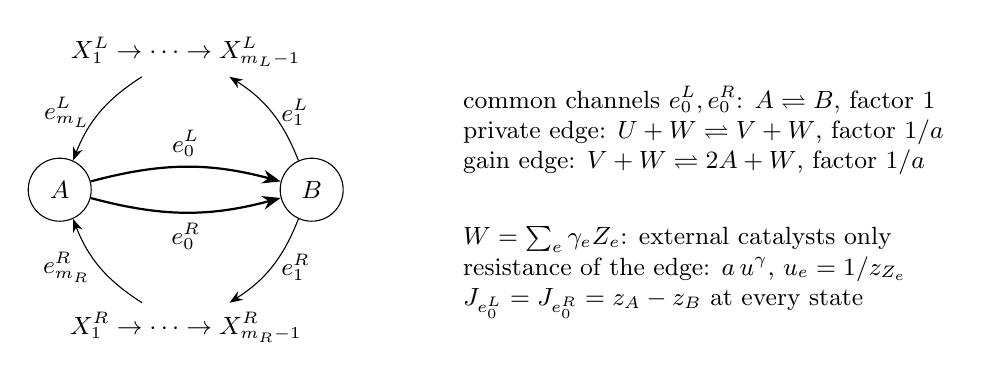
\begin{tikzpicture}[>=Stealth,every node/.style={font=\small}]
\node[circle,draw,minimum size=8mm] (A) at (0,0) {$A$};
\node[circle,draw,minimum size=8mm] (B) at (3.2,0) {$B$};
\node (L) at (1.6,1.75) {$X^L_1\to\cdots\to X^L_{m_L-1}$};
\node (R) at (1.6,-1.75) {$X^R_1\to\cdots\to X^R_{m_R-1}$};
\draw[->,thick] (A) to[bend left=15] node[above,pos=.5] {$e_0^L$} (B);
\draw[->,thick] (A) to[bend right=15] node[below,pos=.5] {$e_0^R$} (B);
\draw[->] (B) to[bend right=18] node[right] {$e_1^L$} (L);
\draw[->] (L) to[bend right=18] node[left] {$e_{m_L}^L$} (A);
\draw[->] (B) to[bend left=18] node[right] {$e_1^R$} (R);
\draw[->] (R) to[bend left=18] node[left] {$e_{m_R}^R$} (A);
\node[align=left,anchor=west] at (5,.75) {common channels $e_0^L,e_0^R$: $A\rev B$, factor $1$\\ private edge: $U+W\rev V+W$, factor $1/a$\\ gain edge: $V+W\rev2A+W$, factor $1/a$};
\node[align=left,anchor=west] at (5,-1.05) {$W=\sum_e\gamma_eZ_e$: external catalysts only\\ resistance of the edge: $a\,u^\gamma$, $u_e=1/z_{Z_e}$\\ $J_{e_0^L}=J_{e_0^R}=z_A-z_B$ at every state};
\end{tikzpicture}
\caption{The two-core source. Arrows show the prescribed orientation of each reversible channel. Every private edge carries its own catalyst complex. A path of length one goes directly from $B$ to $2A$.}
\label{fig:source}
\end{figure}

\subsection{Monomial resistances and polynomial comparison}

Write a sparse polynomial as $g(u)=\sum_{i=1}^Nc_iu^{\gamma_i}$ with rational $c_i$ and exponent vectors $\gamma_i\in\N^d$. Repeated monomials and zero coefficients are allowed. Define
\begin{equation}\label{eq:split}
 P(u)=\sum_{i=1}^N(|c_i|+1)\,u^{\gamma_i},\qquad Q(u)=\sum_{i=1}^N(c_i+|c_i|+1)\,u^{\gamma_i}.
\end{equation}
Every listed coefficient is at least one, and $Q-P=g$. When $N=0$ both are the zero polynomial. The split puts a term at every listed monomial on both branches, so no case distinction on signs is needed.

\begin{lemma}[Literal monomial resistances]\label{lem:monomial}
Introduce external species $Z_1,\ldots,Z_d$ and put $u_e=1/z_{Z_e}$. A private edge padded by $W=\sum_e\gamma_eZ_e$ on both sides and given factor $b=1/a$, with $a>0$, has resistance $a\,u^{\gamma}$.
\end{lemma}

\begin{proof}
By \eqref{eq:current}, $J=\frac1a\prod_ez_{Z_e}^{\gamma_e}(x_{\rm tail}-x_{\rm head})=(x_{\rm tail}-x_{\rm head})/(a\,u^\gamma)$, where $x_{\rm head}=z_A^2$ on the gain edge. The catalysts cancel from the stoichiometric column but not from the current.
\end{proof}

For $K>0$ emit two private paths. The left path has one \emph{offset edge} of resistance $K$ followed by one edge of resistance $(|c_i|+1)u^{\gamma_i}$ for each $i$. The right path has one offset edge of resistance $K/2$ followed by one edge of resistance $(c_i+|c_i|+1)u^{\gamma_i}/2$ for each $i$. The corresponding factors are $1/K$, $2/K$, $1/(|c_i|+1)$ and $2/(c_i+|c_i|+1)$. Thus
\begin{equation}\label{eq:comparator}
 R_L=K+P(u),\qquad R_R=\frac{K+Q(u)}{2},
\end{equation}
and each branch has $N+1$ private edges and $N$ private intermediate species.

\begin{proposition}[Polynomial comparator]\label{prop:comparator}
At external activities $u_e=1/z_{Z_e}>0$ and offset $K>0$, the emitted two-core source is jointly compatible if and only if
\begin{equation}\label{eq:comparison}
 g(u)>0\qquad\text{and}\qquad Q(u)<3K+4P(u).
\end{equation}
Both supplied motifs are PACs, whatever $g$, $K$ and $u$ are.
\end{proposition}

\begin{proof}
Substitute \eqref{eq:comparator} into \eqref{eq:overlap}. The inequality $R_L<2R_R$ reads $K+P<K+Q$, that is $g>0$. The inequality $R_R<2R_L$ reads $K+Q<4K+4P$. The PAC statement is Lemma~\ref{lem:pac}.
\end{proof}

The case $g(u)=0$ is a tangency of the two open intervals and is rejected (Figure~\ref{fig:intervals}).

\begin{figure}[t]
\centering
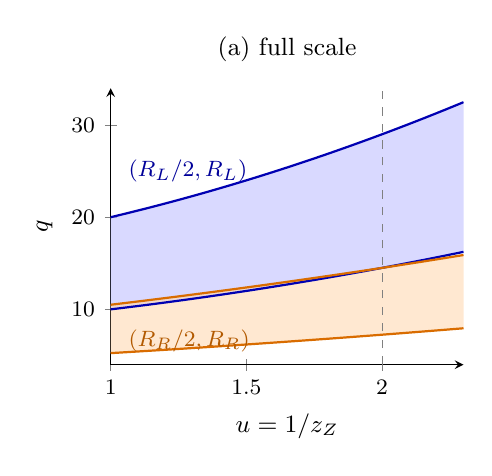
\begin{tikzpicture}
\begin{axis}[width=.5\linewidth,height=.42\linewidth,xmin=1,xmax=2.3,ymin=4,ymax=34,
  xlabel={$u=1/z_{Z}$},ylabel={$q$},title={\small(a) full scale},
  axis lines=left,tick label style={font=\footnotesize},label style={font=\small}]
\addplot[name path=Lhi,draw=blue!70!black,thick,domain=1:2.3,samples=60] {15+3*x+2*x^2};
\addplot[name path=Llo,draw=blue!70!black,thick,domain=1:2.3,samples=60] {(15+3*x+2*x^2)/2};
\addplot[name path=Rhi,draw=orange!85!black,thick,domain=1:2.3,samples=60] {(15+5*x+x^2)/2};
\addplot[name path=Rlo,draw=orange!85!black,thick,domain=1:2.3,samples=60] {(15+5*x+x^2)/4};
\addplot[blue!25,opacity=.6] fill between[of=Lhi and Llo];
\addplot[orange!30,opacity=.6] fill between[of=Rhi and Rlo];
\draw[dashed,gray] (axis cs:2,4) -- (axis cs:2,34);
\node[font=\footnotesize,anchor=west,blue!60!black] at (axis cs:1.03,25) {$(R_L/2,R_L)$};
\node[font=\footnotesize,anchor=west,orange!70!black] at (axis cs:1.03,6.6) {$(R_R/2,R_R)$};
\end{axis}
\end{tikzpicture}\hfill
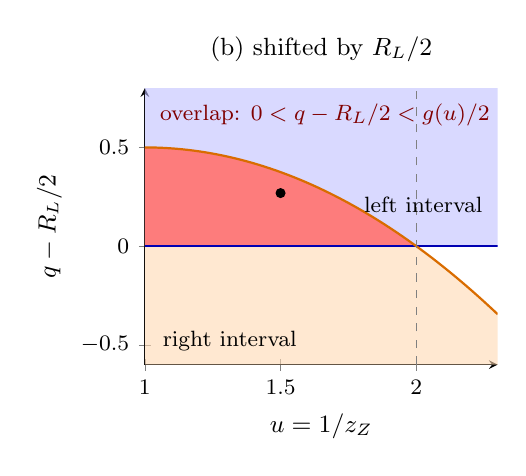
\begin{tikzpicture}
\begin{axis}[width=.5\linewidth,height=.42\linewidth,xmin=1,xmax=2.3,ymin=-0.6,ymax=0.8,
  xlabel={$u=1/z_{Z}$},ylabel={$q-R_L/2$},title={\small(b) shifted by $R_L/2$},
  axis lines=left,tick label style={font=\footnotesize},label style={font=\small},
  yticklabel style={/pgf/number format/fixed}]
\addplot[name path=top,draw=none,domain=1:2.3] {0.8};
\addplot[name path=zero,draw=blue!70!black,thick,domain=1:2.3] {0};
\addplot[name path=bot,draw=none,domain=1:2.3] {-0.6};
\addplot[name path=Rtop,draw=orange!85!black,thick,domain=1:2.3,samples=60] {x-x^2/2};
\addplot[blue!25,opacity=.6] fill between[of=top and zero];
\addplot[orange!30,opacity=.6] fill between[of=Rtop and bot];
\addplot[red!55,opacity=.9] fill between[of=Rtop and zero,soft clip={domain=1:2}];
\draw[dashed,gray] (axis cs:2,-0.6) -- (axis cs:2,0.8);
\node[font=\footnotesize,anchor=south east] at (axis cs:2.28,0.12) {left interval};
\node[font=\footnotesize,anchor=south west] at (axis cs:1.03,-0.58) {right interval};
\node[font=\footnotesize,red!50!black,anchor=south west] at (axis cs:1.02,0.56) {overlap: $0<q-R_L/2<g(u)/2$};
\addplot[only marks,mark=*,mark size=1.6pt] coordinates {(1.5,0.26878612716763)};
\end{axis}
\end{tikzpicture}
\caption{Response intervals of the two cores in the example of Section~\ref{sec:example}, drawn to scale: $g(u)=2u-u^2$, $K=15$, $R_L=15+3u+2u^2$ and $R_R=(15+5u+u^2)/2$. (a) The left interval $(R_L/2,R_L)$ and the right interval $(R_R/2,R_R)$. (b) The same intervals near their overlap, shifted by $R_L/2$: the upper end of the right interval is then $R_R-R_L/2=g(u)/2$. The intervals overlap exactly where $g(u)>0$, touch at $u=2$ where $g=0$, and separate for $u>2$ (outside the box, dashed line, shown for illustration). The dot is the exact state of Section~\ref{sec:example}, with $q=4245/346$.}
\label{fig:intervals}
\end{figure}

\subsection{Fixed boxes}

On $u\in[1,2]^d$ choose the rational constant
\begin{equation}\label{eq:K}
 K=1+\sum_{i=1}^N(c_i+|c_i|+1)\,2^{|\gamma_i|},\qquad|\gamma|=\textstyle\sum_e\gamma_e .
\end{equation}
Then $Q(u)\le K-1<K$ on the box, so the second inequality in \eqref{eq:comparison} holds automatically.

\begin{proposition}[Boxed source]\label{prop:boxed}
With $K$ as in \eqref{eq:K}, external boxes $[1/2,1]$ and internal boxes $[1/4,1/2]$,
\begin{equation}\label{eq:boxediff}
 \exists u\in[1,2]^d:\ g(u)>0\quad\Longleftrightarrow\quad\text{the emitted boxed two-core instance is a YES instance.}
\end{equation}
\end{proposition}

\begin{proof}
A compatible state has $z_{Z_e}\in[1/2,1]$, hence $u=1/z_Z\in[1,2]^d$, and Proposition~\ref{prop:comparator} gives $g(u)>0$. This direction does not use the internal boxes. Conversely, given $u\in[1,2]^d$ with $g(u)>0$, set $z_{Z_e}=1/u_e\in[1/2,1]$. Both inequalities in \eqref{eq:comparison} hold, and the reconstruction in Lemma~\ref{lem:response} places every internal activity in $[1/4,1/2]$.
\end{proof}

All boxes have positive width, and no coordinate is fixed by a singleton box.

\subsection{Positive activities without boxes}

On the positive orthant no constant bounds $Q$. Instead introduce one further external species $Z_0$ and use it as the padding of both offset edges, with factor $1$ on the left and $2$ on the right. By Lemma~\ref{lem:monomial} their resistances are $K=1/z_{Z_0}$ and $K/2$. The offset is thus an activity, chosen existentially like every other activity. It is not a factor selected after a witness is known.

\begin{proposition}[Unboxed source]\label{prop:unboxed}
\begin{equation}\label{eq:unboxediff}
 \exists u\in\R^d_{>0}:\ g(u)>0\quad\Longleftrightarrow\quad\text{the emitted unboxed two-core instance is a YES instance.}
\end{equation}
\end{proposition}

\begin{proof}
A compatible state gives $g(u)>0$ at $u=1/z_Z$ by Proposition~\ref{prop:comparator}. Conversely, if $g(u)>0$, take $K=1+Q(u)$ and $z_{Z_0}=1/K$. Then $Q<K\le3K+4P$, and Proposition~\ref{prop:comparator} applies.
\end{proof}

\section{Proof of the classification}\label{sec:complexity}

\begin{fact}[Schaefer and Štefankovič {\citep[Propositions~2.6 and~2.12]{schaefer2024}}]\label{fact:sources}
The following problems are $\ER$-complete. The input is a polynomial $f\in\Z[x_1,\ldots,x_d]$ given by the explicit list of its monomials with binary integer coefficients.
\begin{enumerate}[label=\textup{(\alph*)}]
\item \emph{Bounded:} $\deg f\le4$; is there $x\in(-1,1)^d$ with $f(x)>0$?
\item \emph{Unbounded:} $\deg f\le6$; is there $x\in\R^d$ with $f(x)>0$?
\end{enumerate}
\end{fact}

These are the one-block, existential cases of the cited propositions, with $\Sigma_1\R=\ER$. The source states them with $f(x)<0$; replacing $f$ by $-f$ gives the form above. At fixed degree, the explicit monomial list has polynomial length.

\begin{lemma}[Closing the cube]\label{lem:closing}
For a continuous $f:[-1,1]^d\to\R$, there is $x\in(-1,1)^d$ with $f(x)>0$ if and only if there is $x\in[-1,1]^d$ with $f(x)>0$.
\end{lemma}

\begin{proof}
One direction is inclusion. If $f(x)>0$ at a point of the closed cube, then $(1-t)x\in(-1,1)^d$ for $0<t<1$, and continuity gives $f((1-t)x)>0$ for small $t>0$. For $d=0$ both sides are the same statement.
\end{proof}

This is a statement about the existence verdict; a boundary witness need not itself lie in the open cube. It allows the boxed reduction to use closed boxes without auxiliary range-enforcement cores.

\begin{proof}[Proof of Theorem~\ref{thm:main}: hardness]
\emph{Boxed.} Let $f$ be an instance of Fact~\ref{fact:sources}(a) and put $g(u)=f(2u-3)$. The affine map $u\mapsto2u-3$ sends $[1,2]^d$ onto $[-1,1]^d$, so Lemma~\ref{lem:closing} shows that $f>0$ somewhere on $(-1,1)^d$ exactly when $g>0$ somewhere on $[1,2]^d$. Expand $g$ into its monomials, with degree at most four, and apply Proposition~\ref{prop:boxed}.

\emph{Unboxed.} Let $f$ be an instance of Fact~\ref{fact:sources}(b) and put $g(u,v)=f(u-v)$ in $2d$ positive variables. Every $x\in\R^d$ equals $u-v$ with $u,v>0$, for example $u_e=\max(x_e,0)+1$ and $v_e=\max(-x_e,0)+1$. Conversely every positive pair defines a real point. Hence $f>0$ somewhere on $\R^d$ exactly when $g>0$ somewhere on $\R^{2d}_{>0}$. Expand $g$, with degree at most six, and apply Proposition~\ref{prop:unboxed}.

\emph{Size.} A monomial of degree $D$ expands under either substitution into at most $\prod_e(\gamma_e+1)\le2^{D}$ monomials, with integer multipliers of absolute value at most $5^D$. Here $D\le4$ or $D\le6$ is a constant, so collecting terms increases coefficient bit lengths by $O(\log(N+1))$. Let $N$ be the number of expanded terms. The coefficients in \eqref{eq:split}, the offset \eqref{eq:K} and the factors (reciprocals of positive rationals) all have polynomial bit length. Table~\ref{tab:size} lists the emitted objects; all are written explicitly with dense complexes and still have polynomial total length. The emitter runs in polynomial time.

\emph{Molecularity and factors.} A private edge carries at most $D$ catalyst units and at most two internal units, giving side molecularity at most $D+2$, that is six in the boxed and eight in the unboxed case. The unboxed offset edges have side molecularity at most three, and the common channels one. Every factor is $1$, $1/K$, $2/K$, $1/(|c|+1)$ or $2/(c+|c|+1)$. Since $K\ge1$ and $|c|+1\ge1$, and $c+|c|+1\ge1$, every factor lies in $(0,2]$.

\emph{Promise.} By Proposition~\ref{prop:comparator} both supplied motifs are PACs in every output, whether the source instance is a YES or a NO instance. An empty or identically zero polynomial produces two valid cycles whose intervals touch, $R_L=K=2R_R$, and hence a NO instance.
\end{proof}

\begin{table}[t]
\centering\small
\begin{tabular}{@{}lll@{}}\toprule
 & closed boxes & positive orthant\\\midrule
hard source (Fact~\ref{fact:sources}) & $\exists x\in(-1,1)^d$, $f(x)>0$, $\deg f\le4$ & $\exists x\in\R^d$, $f(x)>0$, $\deg f\le6$\\
substitution & $x=2u-3$, $u\in[1,2]^d$ & $x=u-v$, $u,v\in\R^d_{>0}$\\
polynomial variables & $d$ & $2d$\\
expanded terms $N$ & $\le16$ per monomial of $f$ & $\le64$ per monomial of $f$\\
supplied cores & $2$ & $2$\\
reaction indices & $2N+4$ & $2N+4$\\
internal species & $2N+2$ & $2N+2$\\
external species & $d$ & $2d+1$ (including $Z_0$)\\
boxes & internal $[1/4,1/2]$, external $[1/2,1]$ & none\\
maximum side molecularity & $6$ & $8$\\
kinetic factors & rationals in $(0,2]$ & rationals in $(0,2]$\\\bottomrule
\end{tabular}
\caption{The two emitted instances. The count of reaction indices includes the two common channels; the two cores share the species $A,B$ and the catalysts, but no reaction index.}
\label{tab:size}
\end{table}

\begin{lemma}[Membership]\label{lem:membership}
Total joint feasibility, the language \JC\ of Definition~\ref{def:jc} without any minimality requirement, belongs to $\ER$.
\end{lemma}

\begin{proof}
Given an instance, write an existential formula over the reals as follows. Introduce a variable $z_s$ and the constraint $z_s>0$ for each species, and the box inequalities where present. Singleton boxes become equations. For each used reaction compute both monomials $\act^{\alpha_r}$ and $\act^{\beta_r}$ by a multiplication circuit. A power $z^a$ with binary exponent $a$ needs $O(\log(a+1))$ gates by repeated squaring, and the powers are then multiplied together. Introduce one real variable $y$ and one equation $y=vw$ for each gate. In a topological order of the circuit, these equations force every gate variable to its intended value. Append the orientation inequalities $\sigma_rb_r(M_{\alpha_r}-M_{\beta_r})>0$ and, for each motif and each of its species, the production inequality $\sum_{r\in T_k}N_{sr}b_r(M_{\alpha_r}-M_{\beta_r})>0$, after clearing positive denominators. The formula has length polynomial in the input, including when exponents are large. It is true exactly when the instance is a YES instance. Its construction takes polynomial time.
\end{proof}

\begin{proof}[Proof of Theorem~\ref{thm:main}: membership and completeness]
The language \JC\ of Lemma~\ref{lem:membership} contains every YES instance of \PJC\ and no NO instance of it, so \PJC\ belongs to $\ER$ in the sense of Definition~\ref{def:promise}. The hardness reductions map YES instances of an $\ER$-complete problem to YES instances of \PJC\ and NO instances to NO instances, and they never leave the promise.
\end{proof}

\begin{remark}[Recognizing the annotations]\label{rem:recognition}
Consider the language of instances in which every supplied motif \emph{is} a PAC and which are compatible. It is $\ER$-hard by the same reduction. It is the intersection of the language \JC, which lies in $\ER$, with the language of valid PAC annotations. The latter lies in coNP. A non-PAC is either not side-incident, which is checked directly, or not productive, which is a linear program, or it has a strict side-incident productive submotif. A certificate for the last case is the pair $(U',T')$, verified by a linear program. The intersection therefore lies in PSPACE \citep{canny1988}. Whether this intersection lies in $\ER$ remains open; containment of coNP in $\ER$ is not known. PAC recognition is a separate decision problem.
\end{remark}

\section{Refinements and consequences}\label{sec:consequences}

Throughout this section \emph{emitted instance} means an output of the reductions in Section~\ref{sec:complexity}.

\subsection{What every output satisfies}

\begin{proposition}[Output properties]\label{prop:outputs}
Every emitted instance, whether YES or NO, has the following properties.
\begin{enumerate}[label=\textup{(\alph*)}]
\item Both supplied motifs are PACs.
\item It is flux feasible: one signed flux, positive on every reaction, makes both cores productive.
\item It is direction feasible: some positive state, inside the boxes in the boxed setting, makes every current positive.
\item $\act=\one$ is an equilibrium at which every current vanishes.
\item Every factor lies in $(0,2]$, and every catalyst has zero net stoichiometric change in every reaction.
\end{enumerate}
Consequently \PJC\ remains $\ER$-hard on instances that satisfy both linear relaxations of Proposition~\ref{prop:relaxations}.
\end{proposition}

\begin{proof}
(a) is Lemma~\ref{lem:pac}. (b) Use $j_0=1$ on both common channels and, independently on each branch of length $m$, $j_i=1-i/[2(m+1)]$; the reaction sets are disjoint. (c) Take $z_A=1/2$, $z_B=3/8$, all catalysts equal to one, and on each branch intermediates strictly decreasing from $3/8$ towards $1/4=z_A^2$. Positive catalysts multiply the drops without changing their signs. (d) Both monomials equal one. (e) was shown in the proof of Theorem~\ref{thm:main}; catalysts occur equally on both sides.
\end{proof}

\subsection{Union production}

Joint compatibility asks for production in each supplied core separately. It does not ask that every species grow under the sum of all reactions, and in general the two requirements differ (Remark~\ref{rem:merged}). For the emitted instances, every compatible state has positive union production.

\begin{proposition}[Positive union production]\label{prop:union}
At every compatible state of an emitted instance, every internal species has strictly positive net production under the union of all reactions, and every external catalyst has zero net production.
\end{proposition}

\begin{proof}
Let $j_0=z_A-z_B$ be the common current and $j^L_i$, $j^R_i$ the private currents. The union productions are
\[
 A:\ (2j^L_{m_L}-j_0)+(2j^R_{m_R}-j_0),\qquad B:\ (j_0-j^L_1)+(j_0-j^R_1),
\]
and each private species receives only its own core's production. Every bracket is a per-core production and is positive. Catalysts occur on both sides of every reaction in which they occur.
\end{proof}

Thus hardness persists if positive union production is added to the compatibility predicate: YES instances satisfy the strengthened predicate, NO instances have no compatible state at all, and membership is unchanged. This does not show hardness of a problem that asks for union production \emph{instead of} per-core production.

\subsection{No parallel channels}

The two common channels have identical complexes and identical factors. They can be merged.

\begin{corollary}[A single shared channel]\label{cor:merged}
Theorem~\ref{thm:main} holds for instances in which no two reaction indices have the same pair of complexes, in either order. The two supplied cores then share exactly one reaction, the channel $A\rev B$.
\end{corollary}

\begin{proof}
Before splitting, append the explicitly listed zero term $0\cdot u^{0}$ to $g$. This leaves $g$ unchanged, adds the constant $1$ to both $P$ and $Q$, increases the boxed offset \eqref{eq:K} by one, and guarantees $N\ge1$. Every private path then has at least one private intermediate. Replace the two common channels by one index $e_0:A\rev B$ with factor one, included in both motifs. Its current equals $z_A-z_B$, the current of each former copy, at every state. Each motif is still literally a gain-two cycle, so it is a PAC by Lemma~\ref{lem:pac}. Every orientation and production inequality is unchanged, so the compatible states are the same.

No two indices now have the same complexes. Every private edge of the left branch has a left-private intermediate on at least one side, since $N\ge1$, and similarly on the right, so no left edge equals a right edge. Within a branch the ordered pairs of internal endpoints of the edges are pairwise different and never reversed, and no private edge equals $A\rev B$ or its reverse. Box widths, factors and molecularity bounds are unchanged.
\end{proof}

\begin{remark}[Per-core versus union production]\label{rem:merged}
After merging, the union production at $B$ is $j_0-j^L_1-j^R_1$. Each private first current exceeds $j_0/2$ by \eqref{eq:chain}, so this is negative at every compatible state, although both cores produce $B$. In the merged variant, per-core compatibility and union growth are therefore genuinely different predicates.
\end{remark}

\subsection{A conservative, food-driven realization}

The gain edges $V+W\to2A+W$ create internal mass, so the emitted networks admit no positive conservation law involving the internal species. An explicit food species removes this without changing any decision.

\begin{proposition}[Food adapter]\label{prop:food}
Add an external species $F$. Replace each common channel and each ordinary private edge $U+W\rev V+W$ by $U+F+W\rev V+F+W$, and each gain edge $V+W\rev2A+W$ by $V+F+W\rev2A+W$, keeping all factors and motifs. Then:
\begin{enumerate}[label=\textup{(\alph*)}]
\item the vector that gives mass one to $F$ and to every internal species, and any positive mass to each catalyst, is conserved by every reaction, and $\act=\one$ is an equilibrium;
\item both motifs are still PACs, and side molecularity is still at most $D+2$;
\item for $\varphi=z_F>0$ and internal activities $z_s=\varphi y_s$, with catalysts unchanged, every current equals $\varphi^2$ times the original current at $y$;
\item hence the unboxed instance is a YES instance exactly when the original is, and the boxed instance with food box $[1,2]$ is a YES instance exactly when the original is.
\end{enumerate}
\end{proposition}

\begin{proof}
(a) Ordinary reactions have internal-plus-food mass $2$ on both sides, and gain reactions have $V+F$ against $2A$. Catalyst masses cancel. (b) $F$ is external, so the internal side incidence and the internal stoichiometric columns are unchanged, and Lemma~\ref{lem:pac} applies. The gain edge's reactant side gains one unit, reaching at most $D+2$. (c) An ordinary current becomes $b\act^W(\varphi y_U\varphi-\varphi y_V\varphi)=\varphi^2b\act^W(y_U-y_V)$, and a gain current becomes $b\act^W(\varphi y_V\varphi-\varphi^2y_A^2)$. (d) Productions are linear in the currents, so every sign condition is preserved in both directions. In the boxed case, completeness uses $\varphi=1$ with the original boxed state. For soundness, divide the internal activities by $\varphi$. The resulting state need not satisfy the internal boxes, but the necessity direction of Proposition~\ref{prop:boxed} used only the external boxes.
\end{proof}

At a compatible state with $\varphi=1$, food is consumed at rate $J^L_{\rm gain}+J^R_{\rm gain}$, which by mass conservation equals the total union production of internal species. Feeding $F$ and withdrawing internal species at these rates balances the state. This is an algebraic balance only; it does not assert stability or startup. The sides of molecularity up to eight are effective mass-action reactions, not claimed to be elementary steps. Replacing them by elementary mechanisms would require a new argument.

\subsection{Families of modules, core count and witness precision}

Several comparators can share their catalysts. Emit, for polynomials $g_1,\ldots,g_k$ in the same variables, one two-core module for each $g_j$. Each module has its own $A_j,B_j$, private species and offset, and all modules share the catalysts $Z_1,\ldots,Z_d$.

\begin{proposition}[Conjunctions]\label{prop:conjunction}
The boxed family of $2k$ supplied PACs is compatible if and only if some $u\in[1,2]^d$ satisfies $g_j(u)>0$ for every $j$. The same holds for the unboxed family, with one offset species $Z_0$ shared by all modules and $u\in\R^d_{>0}$.
\end{proposition}

\begin{proof}
Necessity applies Proposition~\ref{prop:comparator} to each module. For sufficiency, fix $u$, take $K_j$ as in \eqref{eq:K} for each module, or a single $K=1+\max_jQ_j(u)$ in the unboxed case, and reconstruct each module by Lemma~\ref{lem:overlap}. Different modules have disjoint internal species.
\end{proof}

\begin{corollary}[Core count is not a useful parameter]\label{cor:count}
For every fixed $k\ge2$, \PJC\ restricted to instances with exactly $k$ supplied cores is $\ER$-complete, in both settings of Theorem~\ref{thm:main}. Unless $\mathrm P=\ER$, no algorithm runs in polynomial time on the instances with $k$ cores, for any fixed $k\ge2$; in particular there is no algorithm with running time $n^{f(k)}$.
\end{corollary}

\begin{proof}
Add $k-2$ further gain-two cycles of length two, each with its own species and channels and no catalysts. Each is a PAC and is productive on its own by Lemma~\ref{lem:response}, inside the boxes. Being disjoint from the rest, the added cycles change no verdict.
\end{proof}

Strict feasibility always has rational witnesses, because the compatible set is open relative to the box. The next statement shows that such witnesses can be very long.

\begin{proposition}[Doubly exponential denominators]\label{prop:precision}
For $n\ge1$ there is a boxed instance with $2(n+1)$ supplied PACs, side molecularity at most four, factors in $(0,2]$ independent of $n$, and description length $O(n\log n)$ bits, which is a YES instance and in which every compatible state satisfies
\[
 0<1-z_{Z_n}<2^{-2^{n-1}}.
\]
In particular every rational compatible state has $z_{Z_n}=p/q$ with $q>2^{2^{n-1}}$.
\end{proposition}

\begin{proof}
Use variables $u_1,\ldots,u_n\in[1,2]$ and put $v_i=u_i-1\in[0,1]$. Take the modules
\[
 g_0=\tfrac32-u_1,\qquad g_i=u_i^2-2u_i-u_{i+1}+2=v_i^2-v_{i+1}\ \ (1\le i<n),\qquad g_n=u_n-1 .
\]
Their positivity says $v_1<1/2$, $v_{i+1}<v_i^2$ and $v_n>0$. Since $v_i\ge0$, induction gives $0\le v_i<2^{-2^{i-1}}$, so $0<v_n<2^{-2^{n-1}}$. With $z_{Z_n}=1/(1+v_n)$ it follows that $0<1-z_{Z_n}=v_n/(1+v_n)<2^{-2^{n-1}}$. If $z_{Z_n}=p/q<1$ in lowest terms, then $q-p\ge1$, so $1/q\le1-z_{Z_n}$ and $q>2^{2^{n-1}}$. The point $v_i=2^{-(3\cdot2^{i-1}-1)}$ satisfies all constraints, since $v_{i+1}=v_i^2/2$, so the instance is a YES instance by Proposition~\ref{prop:conjunction}. Each module has at most four terms of degree at most two, with coefficients independent of $n$. The squaring modules have offset $K=22$ by \eqref{eq:K}, and every factor lies in $(0,2]$.
\end{proof}

This lower bound concerns ordinary explicitly written rational witnesses. It is consistent with, and illustrates, the fact that membership of \PJC\ in NP would imply $\mathrm{NP}=\ER$.

\section{A worked example in exact arithmetic}\label{sec:example}

Take $d=1$ and $g(u)=2u-u^2$. The split \eqref{eq:split} gives $P=3u+2u^2$ and $Q=5u+u^2$, and \eqref{eq:K} gives $K=1+5\cdot2+1\cdot4=15$. The emitted boxed network has eight reaction indices (Table~\ref{tab:example}). At $u=3/2$, so $z_Z=2/3$, the values are $g=3/4>0$, $R_L=24$ and $R_R=99/8$. The response intervals $(12,24)$ and $(99/16,99/8)$ overlap in $(12,99/8)$.

\begin{table}[t]
\centering\small
\begin{tabular}{@{}llll@{}}\toprule
index & literal reaction & factor & current at the state \eqref{eq:exstate}\\\midrule
$e^L_0$ & $A\rev B$ & $1$ & $173/9182$\\
$e^L_1$ & $B\rev L_1$ & $1/15$ & $89/9182$\\
$e^L_2$ & $L_1+Z\rev L_2+Z$ & $1/3$ & $88/9182$\\
$e^L_3$ & $L_2+2Z\rev2A+2Z$ & $1/2$ & $87/9182$\\
$e^R_0$ & $A\rev B$ & $1$ & $173/9182$\\
$e^R_1$ & $B\rev R_1$ & $2/15$ & $172/9182$\\
$e^R_2$ & $R_1+Z\rev R_2+Z$ & $2/5$ & $171/9182$\\
$e^R_3$ & $R_2+2Z\rev2A+2Z$ & $2$ & $170/9182$\\\bottomrule
\end{tabular}
\caption{The emitted boxed instance for $g(u)=2u-u^2$. The first private edge of each branch is the offset edge; the others realize the terms of $P$ and $Q/2$. The supplied cores are $(\{A,B,L_1,L_2\},\{e^L_0,\ldots,e^L_3\})$ and $(\{A,B,R_1,R_2\},\{e^R_0,\ldots,e^R_3\})$.}
\label{tab:example}
\end{table}

An exact compatible state is
\begin{equation}\label{eq:exstate}
 z_A=\tfrac12,\quad z_B=\tfrac{2209}{4591},\quad z_{L_1}=\tfrac{3083}{9182},\quad z_{L_2}=\tfrac{2687}{9182},\quad z_{R_1}=\tfrac{1564}{4591},\quad z_{R_2}=\tfrac{9947}{36728},\quad z_Z=\tfrac23 .
\end{equation}
All internal activities lie in $[1/4,1/2]$, and $q=4245/346\in(12,99/8)$. The currents are listed in Table~\ref{tab:example}. In units of $1/9182$, the productions of the left core at $A,B,L_1,L_2$ are $(1,84,1,1)$. Those of the right core at $A,B,R_1,R_2$ are $(167,1,1,1)$. The union productions at $A,B,L_1,L_2,R_1,R_2$ are $(168,85,1,1,1,1)$, and the catalyst's is zero, as Proposition~\ref{prop:union} requires. In the food version of Proposition~\ref{prop:food} at $z_F=1$, food is consumed at rate $87+170=257$ in the same units, which equals $168+85+1+1+1+1$.

At the box edge $u=2$ the values are $g=0$, $R_L=29$ and $R_R=29/2$. The intervals $(29/2,29)$ and $(29/4,29/2)$ touch, and no compatible state exists with $z_Z=1/2$. If instead the two common channels are merged (Corollary~\ref{cor:merged}), the per-core productions are unchanged, but the union production at $B$ becomes $(173-89-172)/9182<0$ (Remark~\ref{rem:merged}). The script \texttt{check\_paper.py} in the source package replays every number in this section in exact rational arithmetic. It also exercises the emitter on random small polynomials in both settings.

\section{Formal verification}\label{sec:lean}

The development uses Lean~4.35.0-rc2 and a pinned Mathlib revision \citep{demoura2021,mathlib2020}. The literal network structure \lean{ReversibleCRN}, signed minimality predicate \lean{Motif.IsPAC} and common-state predicate \lean{CoreFamily.MultiCAC} are preserved from the chemical development. The finite rational data model has exactly their reaction currents, stoichiometry and supplied motifs. Its feasibility predicate quantifies one globally shared positive activity vector, and its PAC predicate quantifies all strict species and reaction deletions.

The selected classification statements are \lean{ChemicalCompleteness.boxed_complete} and \lean{ChemicalCompleteness.unboxed_complete} in namespace \lean{JointThermoComplexity.Complexity}. Each states existential-real completeness of an explicit promise problem. The domain requires exactly two valid signed PACs, fixed positive rational factors at most two, the prescribed boxed intervals or no boxes, and maximum side molecularity six or eight. Promise membership is a separating ordinary existential-real language; it does not require recognition of arbitrary PAC annotations. Hardness preserves both source verdicts, so every output, including a NO output, satisfies all these restrictions.

\begin{table}[t]
\centering\small
\begin{tabular}{@{}>{\raggedright\arraybackslash}p{.36\linewidth}>{\raggedright\arraybackslash}p{.58\linewidth}@{}}\toprule
Statement & Lean declarations\\\midrule
Theorem~\ref{thm:main}, boxed and unboxed promise completeness & \lean{ChemicalCompleteness.boxed_complete}, \lean{ChemicalCompleteness.unboxed_complete}\\
Actual binary Turing reduction and all-output promise & \lean{ChemicalCompleteness.reduction_mem_FP}, \lean{etr_reduction}, \lean{output_domain}\\
Total feasibility membership and promise separation & \lean{NetworkFormulaFP.totalFeasibility_mem_ExistsR}, \lean{ChemicalPromiseMembership.member}\\
Exact complete chemical serialization and polynomial time & \lean{DenseCanonicalNetwork.word_code}, \lean{DenseNetworkFP.word_mem_FP}\\
Unconditional strict-positivity source hardness & \lean{StrictSourceHardness.etr_reduction}\\
Both PACs, factors, boxes and side molecularities on both verdicts & \lean{RationalPolynomialPromise.domain}, \lean{RationalLiteralMolecularity.normalized_bounds}\\
Arbitrary-real-coefficient polynomial semantic interfaces & \lean{Emitted.full_boxed_reduction}, \lean{Emitted.full_unboxed_reduction}\\
Structural flux feasibility, union production and factor bounds & \lean{Emitted.family_multiPAC}, \lean{Emitted.compatible_union_production}, \lean{Emitted.boxed_barriers_le_two}, \lean{Emitted.unboxed_barriers_le_two}\\\midrule
Literature facts; LP relaxations and recognition; merged channels, food adapter, fixed-core extensions, witness precision and examples & Cited or conventional proofs; \texttt{check\_paper.py} replays the printed exact arithmetic\\\bottomrule
\end{tabular}
\caption{Formal claim map. The computational declarations use namespace \texttt{JointThermoComplexity.Complexity}; the earlier chemical interfaces retain namespace \texttt{JointThermoComplexity.Emitted}. The two full classification statements are the selected statement-comparison targets.}
\label{tab:lean}
\end{table}

The encodings declare finite dimensions explicitly and retain signed binary coefficients, positive rational factor data, binary exponents and finite membership vectors. An independently specified real-formula language defines existential-real satisfiability. The hardness transducer passes through finite equation systems and degree-four integer strict positivity, with proved coordinate and stored-coefficient bounds in both modes. Quantitative witness and separation bounds discharge the source-hardness bridge. The conventional proof in Section~\ref{sec:complexity} uses the cited degree-restricted facts; the formal classification proves its needed one-block hardness interface directly from the formula language.

The executable chemical representation is an ordered monomial list. Zero coefficients, repeated monomials and repeated variable occurrences are preserved. Its polynomial evaluation is related to the earlier coefficient-list semantics, and the complete emitted bit string is proved equal to the original finite literal-network codec. The reaction numbering, supplied motif membership vectors, prescribed directions and all interval fields are included in this identity. No support enumeration occurs in the binary transducer. The older \lean{PolynomialFrontend} interfaces still allow arbitrary real multivariate polynomials and noncomputable support enumeration: \lean{full_boxed_reduction} uses $x=2v-3$ on $v\in[1,2]^E$, with physical catalyst activities $u_e=1/v_e\in[1/2,1]$; \lean{full_unboxed_reduction} uses $x=u-v$ on the positive orthant. These are separate general semantic interfaces to the same literal construction.

Running time is measured on actual finite-state binary multitape Turing machines. The complete source and network emitters have polynomial transition bounds, not merely polynomial output-length bounds. The membership compiler uses repeated-squaring circuits for binary exponents and maps malformed network strings to a false sentence. The Turing model is adapted from Samuel Schlesinger's Complexitylib; the package attribution records its exact upstream revision and module-system adaptations.

The independent \lean{Challenge} module states the data, semantics, encoding and cost model using only Mathlib imports, followed by the two classification statements. Its deliberate proof holes are confined to theorem proofs and proof-valued codec, inverse-law and positivity fields; all computational definitions are explicit. The \lean{Solution} supplies proved versions. Its selected theorem readbacks use only \texttt{propext}, \texttt{Classical.choice} and \texttt{Quot.sound}. The source package records the selected declarations, exact toolchain and dependency pins, source bindings and verification logs, distinguishing reused strict native evidence from fresh checks.

\section{Scope and open questions}\label{sec:discussion}

The theorem concerns the general literal model: reversible reactions with fixed factors, catalysts that appear on both sides of a reaction, and supplied motifs. Three modelling points deserve emphasis. First, catalysts are shared existential activities, bounded in the boxed variant, and no core is required to produce them. Second, compatibility requires per-core production. For the emitted instances, per-core compatibility implies positive union production of every internal species (Proposition~\ref{prop:union}); the converse need not hold. The merged-channel refinement can have a negative union production even at a compatible state (Remark~\ref{rem:merged}). Third, the result is a statement about one activity vector. No dynamical stability, startup, persistence or operating steady state is asserted, and a failed numerical search does not certify incompatibility.

For practical instances the proof suggests a route rather than a barrier. Once the external activities are fixed or measured, the private paths of these branch assemblies can be eliminated exactly. Feasibility reduces to comparing resistance sums, and the optimal production margin reduces to a small linear program. After this elimination only the external variables remain; with a fixed number of them and fixed degree, general one-block real-algebraic algorithms \citep{basu2014} decide the remaining sentence in time polynomial in the number of terms and their bit sizes. This applies to assemblies of the kind constructed here, not to arbitrary core topologies. The hardness comes from letting the catalyst dependence grow with the input.

The following questions remain open.
\begin{enumerate}[label=(\arabic*)]
\item \emph{Molecularity thresholds.} Is the problem still $\ER$-hard with side molecularity two, or in elementary bimolecular chemistry? The bounds six and eight are what the construction uses; lower bounds on the necessary molecularity are unknown.
\item \emph{Catalyst-free networks.} Without catalysts the resistances of the construction are constants, and the mechanism disappears. Is compatibility of catalyst-free literal cores easier?
\item \emph{Bounded cores.} For weighted two-reaction cores the problem is fixed-parameter tractable in the longest path \citep{fpt2026}. Which bounded-size families of literal cores admit polynomial algorithms?
\item \emph{Recognition.} What is the exact complexity of recognizing PAC annotations, and of the unpromised language of Remark~\ref{rem:recognition}?
\item \emph{Shared channels with union production.} Is the problem hard when parallel channels are forbidden \emph{and} union production is required? Corollary~\ref{cor:merged} and Proposition~\ref{prop:union} give each property separately.
\end{enumerate}

\paragraph{Data and code availability.}
The \LaTeX{} source, the exact replay script \texttt{check\_paper.py}, the independent statement and proved solution, pinned Lean build files and source-bound verification evidence are included in the source package. The Lean development is in \RepoPhrase. The quantitative follow-ups developed alongside this result are recorded separately and are not used in any proof here. They cover exact production margins, robustness to factor uncertainty, and dimensional parameterizations.

\bibliographystyle{plainnat}
\bibliography{refs}

\end{document}

